\documentclass[11pt]{article}
\title{Meccano hexagons gallery}
\author{https://github.com/heptagons/meccano/hexa/gallery}
\date{2023/12/21}

\usepackage{../../meccano}
\usepackage{amssymb}

\begin{document}

\maketitle
\begin{abstract}
We build rigid meccano\meccanoref regular pentagons from sides $4$ to $24$. We restrict all internal strips to remain inside the hexagons's perimeter and don't permit they overlap with others. The internal strips must not be parallel to any side of the hexagon.
\end{abstract}

% 13

\section{Internal strips}

\begin{figure}[h]
\centering
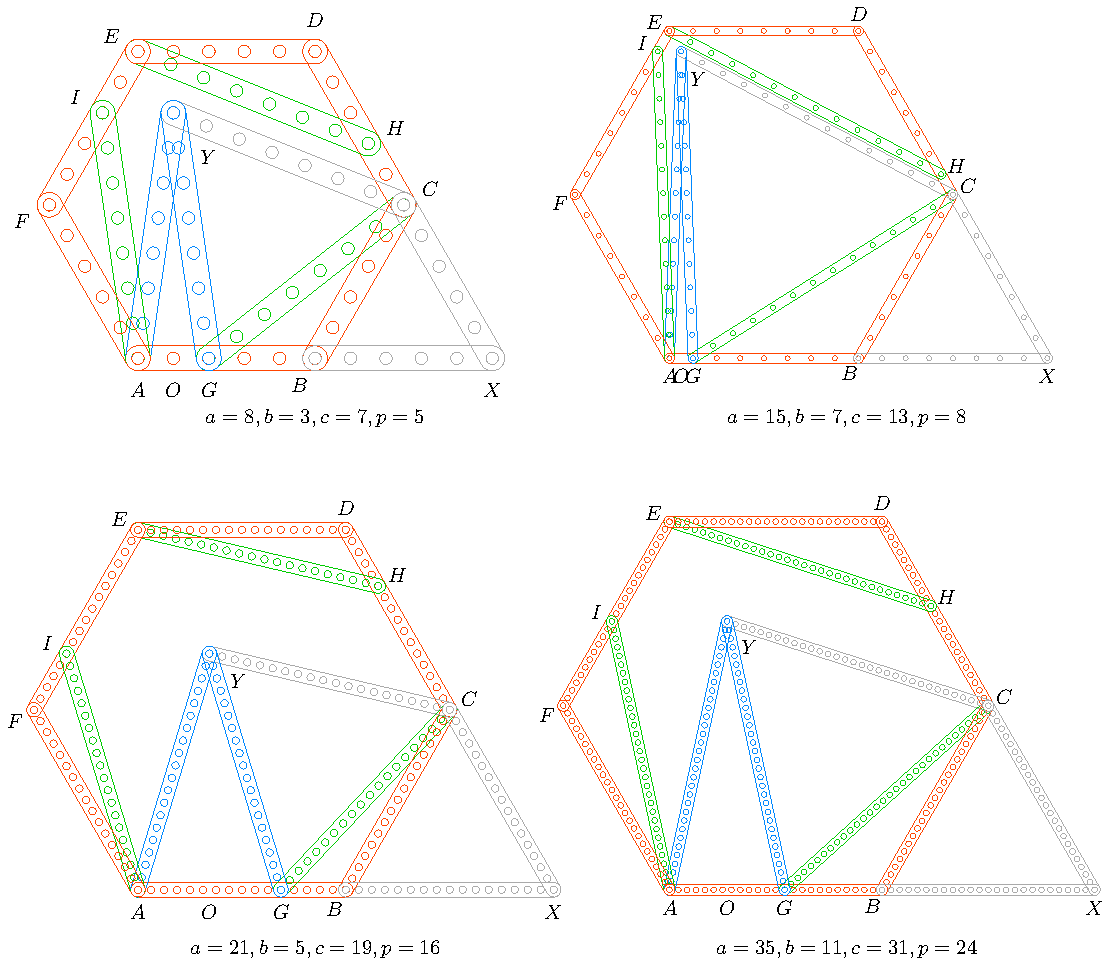
\includegraphics[scale=0.9]{build/hexa-builder-a}
\caption{First four cases where internal strip $c = \overline{GC}$ is an integer and makes rigid two consecutive regular hexagon sides $p = \overline{AB} = \overline{BC}$. We use two numbers to identify every solution $a$ and $b$ where $b = \overline{GB}$ and $a = p - b$ and $c = \sqrt{a^2+b^2-ab}$. }
\label{fig:builder-a}
\end{figure}

We run a software program to look strips that can make rigid two consecutive internal sides of any hexagon. Figure \ref{fig:builder-a} show the smaller four cases found. Consider the figure at top left, the internal hexagon angle is $\theta \equiv \angle{GBC} = 2\pi/3$ and the hexagon side is $p \equiv \overline{BC}$. Consider the triangle $\triangle{GBC}$ and define the other two sides as $b \equiv \overline{GB}$ and $c = \overline{GC}$. By the law of cosines we know that:
\begin{align}
c &= \sqrt{b^2 + p^2 - 2bp\cos\theta} \nonumber\\
 &= \sqrt{b^2 + p^2 - 2bp\left(-\frac{1}{2}\right)} \nonumber\\
 &= \sqrt{b^2 + p^2 + bp}
\end{align}
By defining $a \equiv p + b$ we get:
\begin{align}
c &= \sqrt{a^2 + b^2 - ab} \quad \texttt{ where } a > b
\end{align}

\begin{table}[H]
\begin{center}
\begin{tabular}{||c c c c||} 
 \hline
 $a$ & $b$ & $c$ & $p$ \\ [0.5ex] 
 \hline\hline
  8 &  3 &  7 &  5 \\ \hline
 15 &  7 & 13 &  8 \\ \hline
 21 &  5 & 19 & 16 \\ \hline
 35 & 11 & 31 & 24 \\ \hline
 40 &  7 & 37 & 33 \\ \hline
 48 & 13 & 43 & 35 \\ \hline
\end{tabular}
\caption{Triplets of sides of triangle with angle $2\pi/3$ where $c > p > b$.}
\label{tbl:triplets}
\end{center}
\end{table}

We run a software to iterate first over $0 < a < max$ and then by $1 < b < a$ and filtering $c$ to be integer we get the first rows of triangles with sides $c > p > b$ in table \ref{tbl:triplets}.

Figure $\ref{fig:builder-a}$ shows hexagons of sizes $p = 5,8,16,24$ with perimeter strips in orange made rigid adding three internal green strips of lenght $c = 7,13,19,31$. In the figure we have also an equilateral triangle $\triangle{GCY}$ and an isoscelles triangle $\triangle{AGY}$. The base of the isoscelles triangle is $x \equiv \overline{AG} = \overline{AB} - \overline{GB} = p - b$ and the equals sides $\overline{AY} = \overline{GY} = c$. So we can calculate the height $y \equiv \overline{OY}$:
\begin{align}
y &= \sqrt{(\overline{GY})^2 - (\overline{AO})^2} \nonumber\\
 &= \sqrt{c^2 - \left(\frac{p - b}2\right)^2} \nonumber\\
 &= \sqrt{b^2 + p^2 + bp - \left(\frac{p-b}2\right)^2} = \frac{(p+s)\sqrt3}2 = \frac{a\sqrt3}2
\end{align}



\begin{figure}[H]
\centering
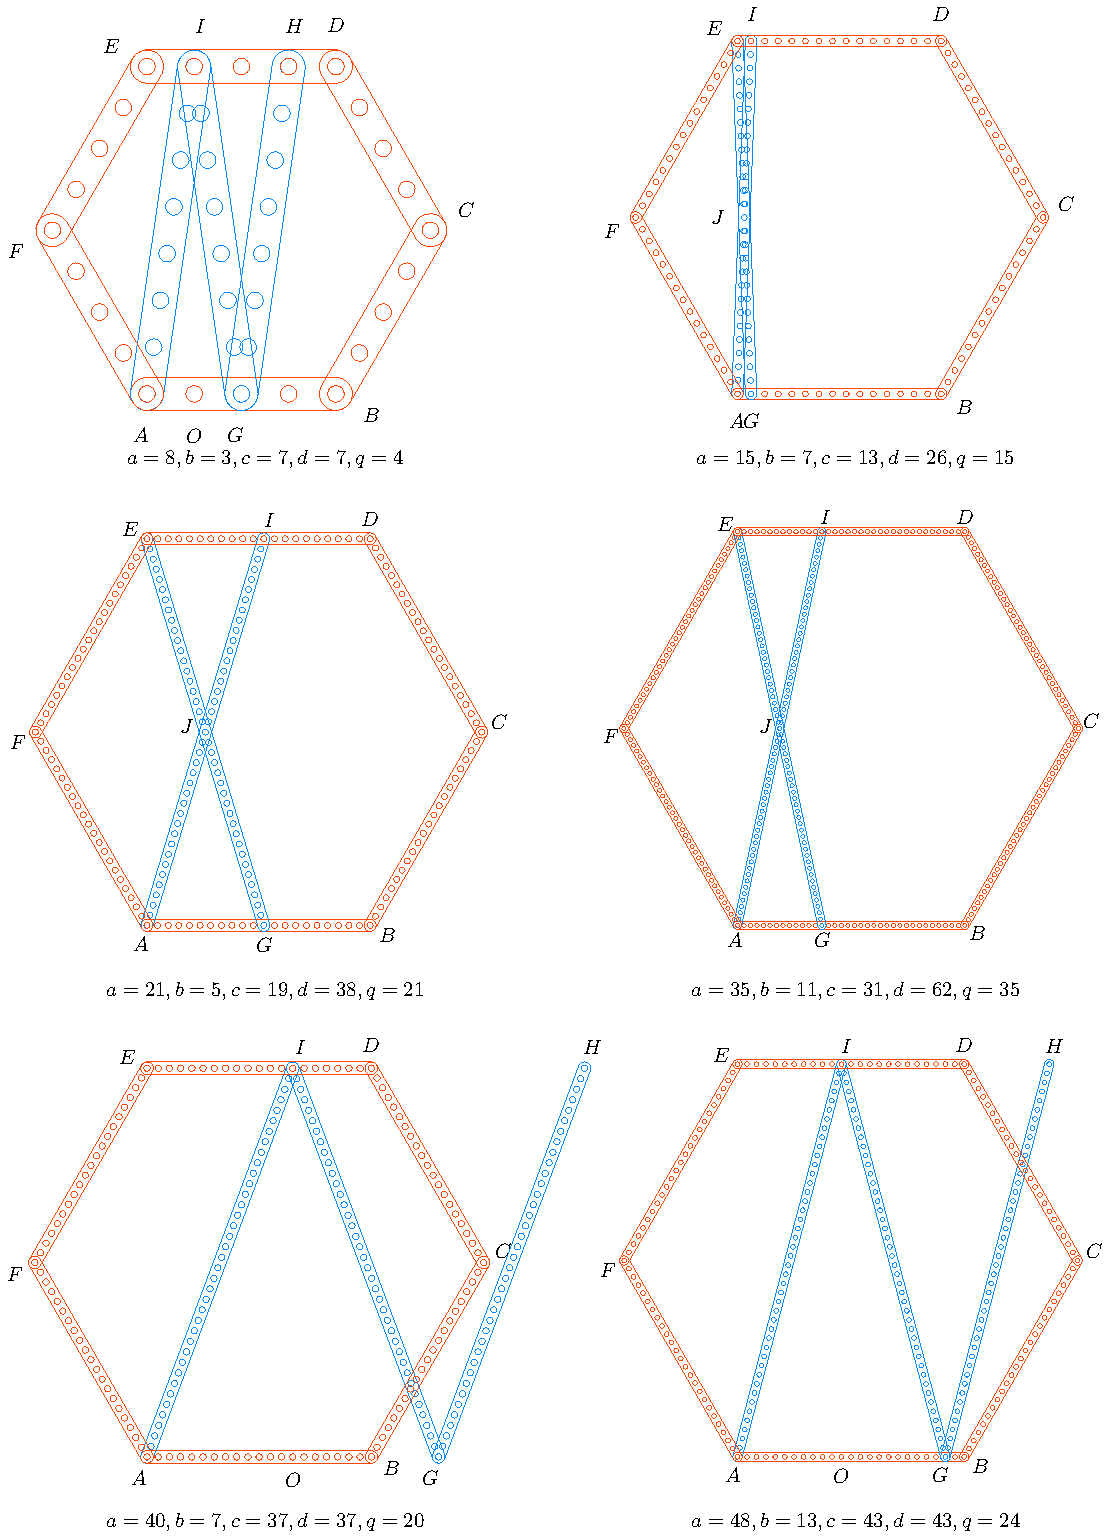
\includegraphics[scale=0.8]{build/hexa-builder-b}
\caption{First six cases of integral distances $c$. When the distance $p-b = \overline{AG}$ is even, we use the strips $d = c$ to join opposites sides of hexagons of side $q = a/2$. When is odd, we use the strips $d = 2c$ to join opposites sides of hexagons of side $q = a$.}
\label{fig:builder-b}
\end{figure}

We know $\dfrac{a\sqrt3}2$ is the height of the regular hexagon of side $\dfrac{a}2$ so we can use the blue strips to connect opposite sides. Figure \ref{fig:builder-b} show the smaller hexagons that have integer strips connecting opposites sides.

Through the gallery we will use the green and blue strips and scaled copies of such strips to make rigid regular hexagons from size $4$ to $24$. We prioritize minimum number of bolts, minimum number of strips and the largest strips sizes as possible.

\section{Hexagons of size 13}

\begin{figure}[H]
\centering
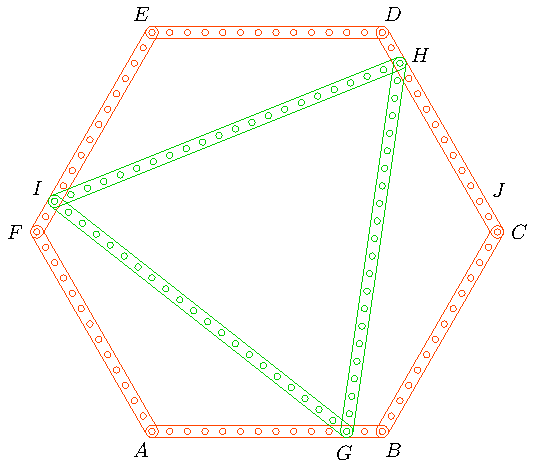
\includegraphics[scale=1]{13/hexa-13a}
\caption{Hexagon of size $s = 13$. Diagonals $c = \overline{GH} = \overline{HI} = \overline{IG} = 21$.}
\label{fig:13a}
\end{figure}

Figure \ref{fig:13a} show hexagon of size $s = 13$. First we detect an offset $o \equiv \overline{DH}$ which we use to calculate the sides $p',b',c'$ of triangle $\triangle{GJH}$:
\begin{align}
o &\equiv \overline{DH} = \overline{CJ} = 2 \nonumber\\
p' &\equiv \overline{GJ} = \overline{BC} + o = 13+2 = 15 \nonumber\\
b' &\equiv \overline{JH} = \overline{CD} - 2o = 13 - 2(2) = 9 \nonumber\\
c' &\equiv \overline{GH} = 21
\end{align}
We confirm triplet $c',p',b'$ is three times ($n=3$) valid hexagonal triplet $c=7,p=5,b=3$.
This case has an equilateral triangle $\triangle{GHI}$ inside the hexagon because is a special of the general case when:
\begin{align}
nb &= s - 2o \nonumber\\
np &= s + o \nonumber\\
nc &= \sqrt{(nb)^2 + (np)^2 - (nb)(np)} \nonumber\\
   &= \sqrt{(s - 2o)^2 + (s+o)^2 + (s - 2o)(s+o)} \nonumber\\
   &= \sqrt{3s^2 - 3so + 3o^2}
\end{align}

First terms of this case is shown in the table \ref{tbl:eqtriangles}
\begin{table}[H]
\begin{center}
\begin{tabular}{||c c c c c||} 
 \hline
 $s$ & $o$ & $c$ & $p$ & $b$ \\ [0.5ex] 
 \hline\hline
%  8 &  3 &  7 &  5 \\ \hline
  13 &  2 &  21 &  15 &  9 \\ \hline
  23 &  1 &  39 &  24 & 21 \\ \hline
  37 & 11 &  57 &  48 & 15 \\ \hline
  59 & 13 &  93 &  72 & 33 \\ \hline
  73 & 26 & 111 &  99 & 21 \\ \hline
  83 & 22 & 129 & 105 & 39 \\ \hline
  94 & 23 & 147 & 117 & 48 \\ \hline
\end{tabular}
\caption{Equilateral triangles side $c$ inside regular hexagons side $s$.}
\label{tbl:eqtriangles}
\end{center}
\end{table}

\section{Hexagon of size $\ge 20$}

\begin{figure}[H]
\centering
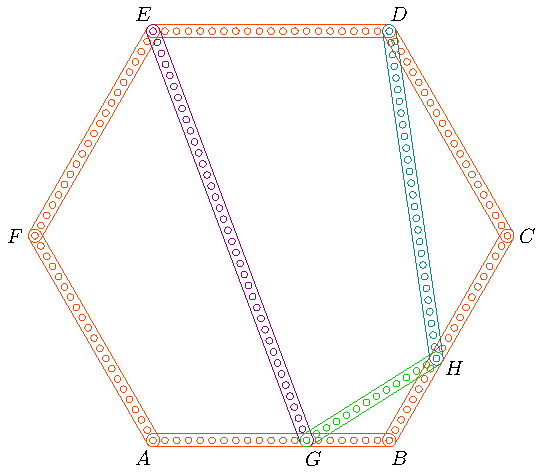
\includegraphics[scale=1]{20/hexa-20a}
\caption{Hexagon of size $20$. The three diagonals needs only two extra bolts at vertices $G$ and $H$. $\overline{GH} = 13$, $\overline{HD} = 28$ and $\overline{EG} = 37$.}
\label{fig:20a}
\end{figure}

Figure \ref{fig:20a} show regular hexagon $ABCDEF$ of size $20$. Triangle $\triangle{GBH}$ sides are $c_1=13,p_1=8,b_1=7$. Triangle $\triangle{HCD}$ sides are $c_2=28,p_2=20,b_2=12$ which is triplet $(7,5,3)$ multiplied by $4$. Right triangle $\triangle{EAG}$ has side $\overline{AE} = \sqrt{(\overline{EG})^2 - (\overline{AG})^2} = \sqrt{37^2 - 13^2} = 20\sqrt3$.


\begin{figure}[H]
\centering
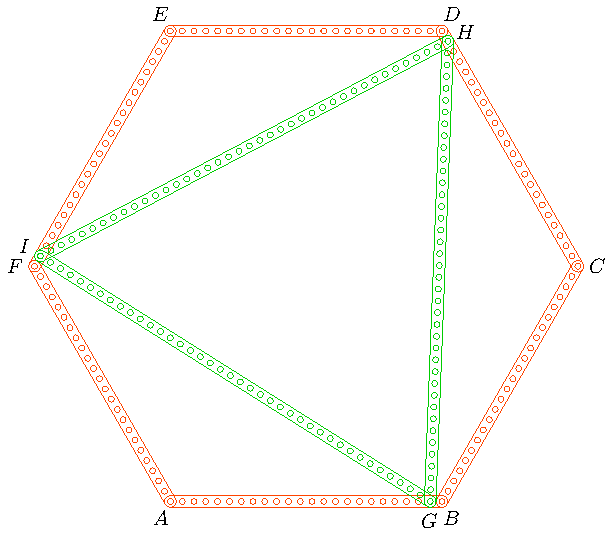
\includegraphics[scale=1]{23/hexa-23a}
\caption{Hexagon of size $s = 23$. Diagonals $c = \overline{GH} = \overline{HI} = \overline{IG} = 39$.}
\label{fig:23a}
\end{figure}

Figure \ref{fig:23a} show a regular hexagon of size $s=23$. Is the second hexagon having an equilateral triangle of size $c=39$ inside as is explained in table \ref{tbl:eqtriangles}.

\begin{figure}[H]
\centering
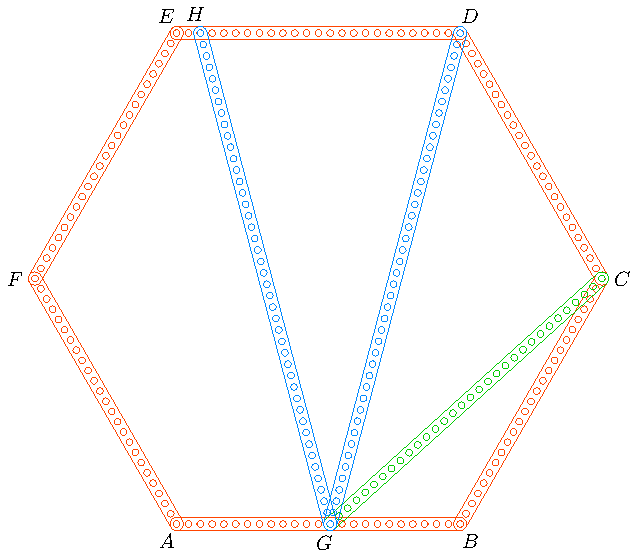
\includegraphics[scale=1]{24/hexa-24a}
\caption{Hexagon of size $s = 24$. Needs only two extra bolts at vertices $G$ and $H$. Diagonal $\overline{GC} = 31$ and diagonals $\overline{GD} = \overline{GH} = 43$. Segments $\overline{GB} = 11$ and $\overline{DH} = 22$.}
\label{fig:24a}
\end{figure}

Figure \ref{fig:24a} show a regular hexagon of size $s = 23$. Triangle $\triangle{GBC}$ has sides $c_1=31, p_1=24, b_1=11$ which is the fourth triplet of table \ref{tbl:triplets}. Triangle $\triangle{DHG}$ is the isoscelles triangle shown in figure \ref{fig:builder-b} case $a=48$.



\end{document}
